\documentclass{article}
\usepackage{iclr2024_conference,times}

\usepackage[utf8]{inputenc} % allow utf-8 input
\usepackage[T1]{fontenc}    % use 8-bit T1 fonts
\usepackage{hyperref}       % hyperlinks
\usepackage{url}            % simple URL typesetting
\usepackage{booktabs}       % professional-quality tables
\usepackage{amsfonts}       % blackboard math symbols
\usepackage{nicefrac}       % compact symbols for 1/2, etc.
\usepackage{microtype}      % microtypography
\usepackage{xcolor}         % colors
\usepackage{wrapfig}
\usepackage{caption}
\usepackage{subcaption}

\usepackage{mymathstyle} % math style with a bunch of commands defined

\usepackage{cleveref}
\usepackage{algorithm2e}
\usepackage{graphicx}
\crefname{algocf}{alg.}{algs.}
\Crefname{algocf}{Algorithm}{Algorithms}
\RestyleAlgo{ruled}

\usepackage{tikz}
\usetikzlibrary{positioning}
\pgfmathtruncatemacro\distance{1}
\usepackage{fp}

\usepackage{mathrsfs}
\RequirePackage{hypernat}
\usepackage{graphicx}
\usepackage{verbatim}

%region custom commands
\newcommand{\softreliprod}[3]{\left\langle #1, #2 \, \vert \, #3 \right\rangle_\mathrm{rel}}
\newcommand{\reliprod}[2]{\left\langle #1, #2 \right\rangle_\mathrm{rel}}
\let\phi\varphi

% commands for comments
\newcommand{\awni}[1]{\textcolor{blue}{\texttt{[Awni]}: #1}}
\newcommand{\john}[1]{\textcolor{red}{\texttt{[John]}: #1}}
%endregion

\interfootnotelinepenalty=10000 % prevent footnote from running over


\title{Relational Convolutional Networks: \\ A framework for learning representations of hierarchical relations}
% The \author macro works with any number of authors. There are two commands
% used to separate the names and addresses of multiple authors: \And and \AND.
%
% Using \And between authors leaves it to LaTeX to determine where to break the
% lines. Using \AND forces a line break at that point. So, if LaTeX puts 3 of 4
% authors names on the first line, and the last on the second line, try using
% \AND instead of \And before the third author name.

\author{Antiquus S.~Hippocampus, Natalia Cerebro \& Amelie P. Amygdale \thanks{ Use footnote for providing further information
about author (webpage, alternative address)---\emph{not} for acknowledging
funding agencies.  Funding acknowledgements go at the end of the paper.} \\
Department of Computer Science\\
Cranberry-Lemon University\\
Pittsburgh, PA 15213, USA \\
\texttt{\{hippo,brain,jen\}@cs.cranberry-lemon.edu} \\
\And
Ji Q. Ren \& Yevgeny LeNet \\
Department of Computational Neuroscience \\
University of the Witwatersrand \\
Joburg, South Africa \\
\texttt{\{robot,net\}@wits.ac.za} \\
\AND
Coauthor \\
Affiliation \\
Address \\
\texttt{email}
}

\begin{document}



\maketitle

\begin{abstract}
    blah
\end{abstract}

\section{Introduction}\label{sec:intro}

Objects in the real world rarely exist in isolation; 
% understanding and 
modeling the relationships between them is essential to accurately capturing complex systems. As increasingly powerful machine learning models progress towards building internal ``world models,'' it is important to explore natural inductive biases to enable efficient learning of relational representations. The computational challenge lies in developing the components necessary for constructing robust, flexible, and progressively complex relational representations.

Compositionality---used here to mean an ability to compose modules together to build iteratively more complex feature representations---is essential to the success of deep representation learning. 
% For example, in a feedforward network, each layer builds on the one before, and in a CNN, each convolution builds an iteratively more complex feature map~\citep{zeiler2014visualizing}. 
For example, CNNs extract higher-level features (e.g., textures and object-specific features) by composing simpler feature maps~\citep{zeiler2014visualizing}, resulting in a flexible architecture for computing ``features of features''.
So far, work on relational representation learning has been limited to ``flat'' first-order architectures. In this work, we propose \textit{\bfseries relational convolutional networks} as a compositional framework for learning hierarchical relational representations.

\begin{wrapfigure}{R}{0.5\textwidth}
    \centering
    \vskip-12pt
    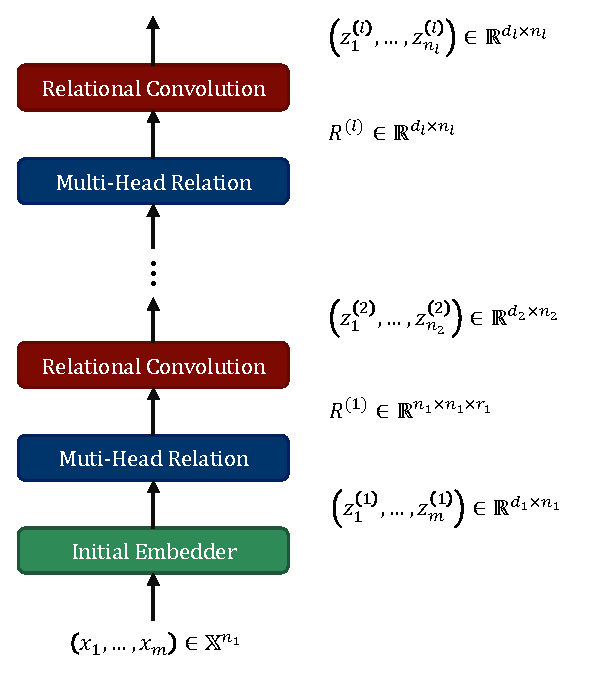
\includegraphics[width=.48\textwidth]{figs/relconv_architecture.pdf}
    \vskip-12pt
    \caption{Proposed architecture for relational convolutional networks. Hierarchical relations are modeled by iteratively computing pairwise relations between objects and convolving the resultant relation tensor with graphlet filters representing templates of relations between groups of objects.
    }\label{fig:relconv_architecture}
    % \vskip-12pt
\end{wrapfigure}

The key to the framework proposed in this paper involves formalizing the concept of convolving learnable templates of a relational pattern against a larger relation tensor. This operation produces a sequence of vectors representing the relational pattern within each group of objects. Crucially, composing relational convolutions captures higher-order relational features---i.e., relations between relations. Specifically, our proposed architecture introduces the following novel concepts and computational mechanisms.
\begin{itemize}%[itemsep=1pt]
    \item \textit{\bfseries Graphlet filters.} A ``graphlet filter'' is a template for the pattern of relations between a (small) collection of objects. 
    Since pairwise relations can be viewed as edges on a graph, the term ``graphlet'' is used to refer to a subgraph, and the term ``filter'' is used to refer to a learnable template or pattern.
    % Graphlet filters are analogous to filters (also called kernels) in traditional CNNs for images, which represent templates for local regions of an image.
    \item \textit{\bfseries Relational convolutions.} 
    We formalize a notion of \textit{relational} convolution, analogous to spatial convolutions in CNNs, where a graphlet filter is matched against the relations within \textit{groups} of objects to obtain a representation of the relational pattern in different groupings of the input.
    % In CNNs for image processing, each filter is
    %  ``swept,'' or 
    % spatially convolved across the image. For relational learning, we formalize an analogous notion of convolution where a graphlet filter can be matched against the relations between each group of objects.
    \item \textit{\bfseries Grouping mechanisms.} For large problem instances, it would be computationally and statistically intractable to consider relational convolutions across all combinations of objects. To achieve scalability, we introduce a learnable grouping mechanism based on attention which identifies the relevant groups that should be considered for the downstream task.
    \item \textit{\bfseries Compositional relational modules.} The proposed architecture supports composable modules, where each module has learnable graphlet filters and groups. This enables learning higher-order relationships between objects---relations between relations.
    % ---that are analogous to the composed feature maps that are of the essence in CNNs.
\end{itemize}


The architecture is presented in detail in Sections~\ref{sec:mdipr} and~\ref{sec:relconv}, and a schematic of the proposed architecture is shown in~\Cref{fig:relconv_architecture}. In a series of experiments, we show how relational convolutional networks provide a powerful framework
% and inductive bias 
for relational learning. We first carry out experiments on the ``relational games'' benchmark for relational reasoning proposed by~\citet{shanahanExplicitlyRelationalNeural}, which consists of a suite of binary classification tasks for identifying abstract relational rules between a set of geometric objects represented as images. 
We next carry out experiments on a version of the \textit{SET} game, which requires processing of higher-order relations across multiple attributes. We find that relational convolutional networks outperform transformers, graph neural networks, as well as existing relational architectures. We argue that these results demonstrate that both compositionality and relational inductive biases are needed to efficiently learn representations of complex higher-order relations.

\subsection{Related Work}\label{ssec:related_work}

To place our framework in the context of previous work, we briefly discuss related forms of relational learning below, pointing first to the review of relational learning inductive biases by~\cite{battagliaRelationalInductiveBiases2018}%,palmRecurrentRelationalNetworks2018,zhangRAVENDatasetRelational2019}. % battaglia is a review of "relational inductive biases" (though in a somewhat different sense to us). the rest are more specific, so this may not be the best place to cite them.

{Graph neural networks} (GNNs) are a class of neural network architectures which operate on graphs and process ``relational'' data~\citep[e.g.,][]{niepertLearningConvolutionalNeural2016,kipfSemiSupervisedClassificationGraph2017,schlichtkrullModelingRelationalData2017,velickovicGraphAttentionNetworks2017,kipfNeuralRelationalInference2018,xuHowPowerfulAre2018}. A defining feature of GNN models is their use of a form of neural message-passing, wherein the hidden representation of a node is updated as a function of the hidden representations of its neighbors on a graph~\cite{gilmerNeuralMessagePassing2017}. Typical examples of tasks which GNNs are applied to include node classification, graph classification, and link prediction~\cite{hamiltonGraphRepresentationLearning2020}. %This is a very general model which includes as a special case convolutional neural networks, where the graph is a grid, and Transformers, where the graph is a complete graph and the message-passing function is a convex sum of the neighbors' representations.

In GNNs, the `relations' are given to the model via edges in a graph. In contrast, our architecture, as well as the explicitly relational architectures described below, operate on collections of objects without any relations given as input. Instead, such relational architectures must infer the relevant relations from the objects themselves. Still, graph neural networks can be applied to these relational tasks by passing in the collection of objects along with a complete graph. % A Transformer Encoder can be thought of as a special case of this architecture.%, and hence is the representative baseline we compare against in our experiments.

Several works have proposed architectures with the ability to model relations by incorporating an {attention mechanism}~\citep[e.g.,][]{vaswani2017attention,velickovicGraphAttentionNetworks2017,santoroRelationalRecurrent2018,zambaldiDeepReinforcementLearning2018,locatelloObjectCentricLearningSlot2020}. Attention mechanisms, such as self-attention in Transformers~\citep{vaswani2017attention}, model relations between objects implicitly as an intermediate step in an information-retrieval operation
% a form of neural message-passing in order 
to update the representation of each object as a function of its context.

There also exists a growing literature on neural architectures which aim to explicitly model relational information between objects. An early example is the relation network proposed by~\citet{santoroSimpleNeural2017}.~\citet{shanahanExplicitlyRelationalNeural} proposes the PrediNet architecture, which aims to learn relational representations which are compatible with predicate logic.
% \todo{removed citation of ESBN for space (since not in baselines). can put back in camera-ready.}
% ~\citet{webbEmergentSymbols2021} proposes ESBN, a recurrent neural network augmented with external memory whose memory-write operation aims to factors representations into `sensory' and `relational'.
~\citet{kergNeuralArchitecture2022} proposes CoRelNet, a simple architecture based on `similarity scores' which aims to distill the relational inductive biases discovered in previous work into a minimal architecture.~\citet{altabaaAbstractorsTransformer2023} explored relational inductive biases in the context of Transformers, and proposed a view of relational inductive biases as a type of selective ``information bottleneck'' which disentangles relational information from object-level features.~\citet{webbRelationalBottleneckInductive2023} provides a cognitive science perspective on this idea, arguing that a relational information bottleneck may be a mechanism for abstraction in the human mind.% and brain.



\section{Multi-dimensional inner product relation module}\label{sec:mhr}

\begin{wrapfigure}{R}{0.5\textwidth}
    \centering
    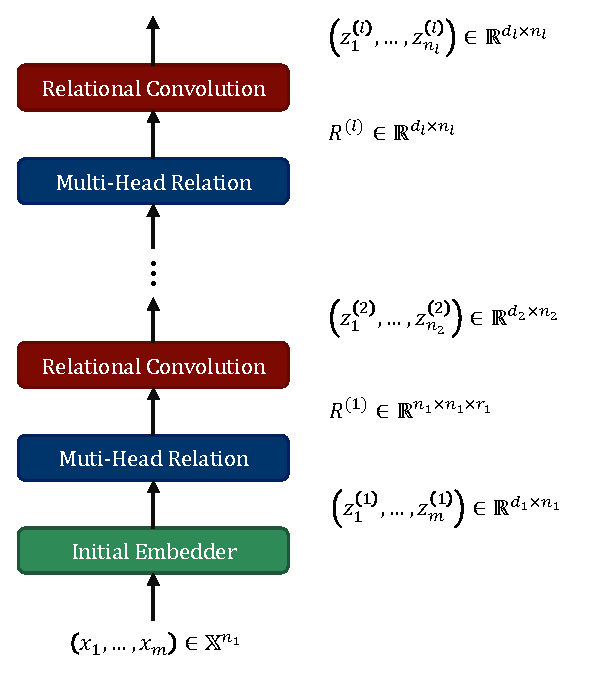
\includegraphics[width=.5\textwidth]{figs/relconv_architecture.pdf}
    \caption{Proposed architecture for relational convolutional networks. Hierarchical relations are modeled by iteratively computing pairwise relations between objects and convolving the resultant relation tensor with graphlet filters representing templates of relations between groups of objects.
    }\label{fig:relconv_architecture}
\end{wrapfigure}
% AWNI: [TODO] UPDATE NOTATION IN THIS FIGURE. E.G., $n$, $n_g^{(l)}$, $d$, $d^{(l)}$ etc.

A relation function is a function that maps a pair of objects $x, y \in \calX$ to a vector representing the relation between the two objects. For example, a relation may represent the information ``$x$ has the same color as $y$'', ``$x$ is larger than $y$'', and ``$x$ is to the left of $y$''. In principle, this can be modeled by an arbitrary learnable function on the concatenation of the two objects' representations. For example,~\citep{santoroSimpleNeural2017} models relations by MLPs applied to the concatenation of pairs of objects. While this approach may work in some cases, it is missing some crucial inductive biases. In particular, there is no constraint that the learned pairwise function is in fact \textit{relational}---it may just as well represent non-relational information like ``$x$ is bright'' and ``$y$ is small.''%, as opposed to relational information like ``$x$ is larger than $y$''.

Recent work has explored using \textit{inner products} to model relations between objects~\citep{webbEmergentSymbols2021, kergNeuralArchitecture2022, altabaaAbstractorsTransformer2023}. The advantage of such an approach is that it provides added pressure to learn explicitly relational representations, disentangling relational information from attributes of individual objects. In particular, it induces a geometry on the object space $\calX$ which allows objects to be described in relation to each other. For example, in the symmetric case, the inner product $\iprod{\phi(x)}{\phi(y)}$ induces a metric on $\calX$. In fact, the relation $\iprod{\phi(x)}{\phi(y)}$ attaches well-defined notions of distance, angles, and orthogonality to the space $\calX$.

More generally, we can allow for multi-dimensional relations by having multiple encoding functions, each extracting a feature to compute a relation on. Furthermore, we can allow for asymmetric relations by having different encoding functions for each object. Hence, we model relations by,
\begin{equation}\label{eq:relation_function}
    r(x, y) = \paren{
        \iprod{\phi_1(x)}{\psi_1(y)},\, \ldots,\, \iprod{\phi_{d_r}(x)}{\psi_{d_r}(y)}} \in \reals^{d_r},
\end{equation}
where $\phi_1, \psi_1, \ldots, \phi_{d_r}, \psi_{d_r}$ are learnable functions. For each dimension of the relation function, the maps $\phi_k, \psi_k$ extract a particular attribute of the objects which is then compared by the inner product.

To promote weight sharing, we can have one common non-linear map $\phi$ across all dimensions along with different linear maps for each object and each dimension of the relation. That is,
\begin{equation}\label{eq:relation_function_lin_proj}
    r(x, y) = \paren{\iprod{W_1^{(1)}\phi(x)}{W_2^{(1)}\phi(y)},\, \ldots,\, \iprod{W_1^{(d_r)}\phi(x)}{W_2^{(d_r)}\phi(y)}},
\end{equation}
where the learnable parameters are $\phi$ and $W_1^{(k)}, W_2^{(k)}, k \in [d_r]$. $\phi: \calX \to \reals^{d_\phi}$ may be an MLP, for example, and $W_1^{(k)}, W_2^{(k)}$ are $d_{\mathrm{proj}} \times d_\phi$ matrices. The class of functions realizable by~\Cref{eq:relation_function_lin_proj} is the same as~\Cref{eq:relation_function} but enables greater weight sharing.

The ``Multi-dimensional Inner Product Relation'' (MD-IPR) module receives a sequence of objects $x_1, \ldots, x_n$ as input and models the pairwise relations between them by~\Cref{eq:relation_function_lin_proj}, returning an $n \times n \times d_r$ relation tensor, $R[i,j] = r(x_i, x_j)$, describing the relations between each pair of objects.

% removed for now.
% \subsection{Universal approximation of inner product relations}
% \awni{todo---post to arxiv and add citation. Also, is statement as a theorem necessary, or should we just state the result in text?}

\citep{arxivInnerprodUnivApprox} analyzes the function class of relation functions on $\calX \times \calX$ realizable by inner products of neural network transformations of the form $\iprod{\phi(x)}{\psi(y)}$. The result implies that when $\phi_i, \psi_i$ are multi-layer perceptrons, $r(x,y)$ in~\Cref{eq:relation_function} can approximate any continuous function from $\calX \times \calX$ to $\reals^{d_r}$ uniformly and with arbitrary precision, provided that $\calX$ is a compact subset of euclidean space.

\begin{theorem}[Theorem 3.1 in~\citep{arxivInnerprodUnivApprox}]
    Suppose $\calX$ is a compact subset of euclidean space. Consider the relation model,
    \begin{equation*}
        \hat{r}(x, y) := \paren{\iprod{\phi_\theta^{(1)}(x)}{\psi_\theta^{(1)}(y)}, \ldots, \iprod{\phi_\theta^{(d_r)}(x)}{\psi_\theta^{(d_r)}(y)}},
    \end{equation*}
    \noindent where $\phi_\theta^{(i)}, \psi_\theta^{(i)}: \calX \to \reals^d$ are multi-layer perceptrons with parameters in $\theta$. Then, for any continuous relation function $r: \calX \times \calX \to \reals^{d_r}$ there exists multi-layer perceptrons with parameters $\theta$ such that $\hat{r}$ approximates $r$ uniformly over $(x,y) \in \calX \times \calX$. Formally, for any $\epsilon > 0$, there exists neural networks with parameters $\theta$ such that,
    \begin{equation*}
        \sup_{x, y \in \calX} \infnorm{r(x,y) - \hat{r}(x,y)} < \epsilon.
    \end{equation*}
\end{theorem}

\section{Relational convolutions with graphlet filters}\label{sec:relconv}

\subsection{Relational convolutions with discrete groups}
Suppose that we have a sequence of objects $(x_1, \ldots, x_n)$ and a relation tensor $R$ describing the pairwise relations between them (obtained by a MD-IPR layer). The relational convolution operation we will define does two things: 1) extracts representations of the relational patterns within \textit{groups} of objects using pairwise relations, and 2) transforms the relation tensor back into a sequence of objects, allowing it be composed with another relational layer to compute higher-order relations.

Fix some filter size $s < n$, where $s$ is a hyperparameter of the relational convolution layer. One `filter' is given by the \textit{graphlet} $f_1 \in \mathbb{R}^{s \times s \times d_r}$. This is a `template' for the pairwise relations between $s$ objects. Note that the dimension of the relations in this filter matches that of the input relation tensor. Let $g \subset [n]$ be a subset of the objects of size $s$. Suppose for now that $g$ is an ordered set (i.e., the group $(1, 2, 3)$ is different from the group $(2, 3, 1)$). Then, denote the relation sub-tensor given by this (ordered) subset by $R[g] := [R[i,j]]_{i,j \in g}$. We define the `relational inner product' between this relation subtensor and the filter $f_1$ by
\begin{equation}
    \label{eq:relational_inner_prod_one_filt}
    \reliprod{R[g]}{f_1} \coloneqq \sum_{i,j \in g} \iprod{R[i,j]}{f_1[i,j]}_{\reals^{d_r}} = \sum_{i,j \in g} \sum_{k \in [d_r]} R[i,j,k] f_1[i,j,k].
\end{equation}
This is simply the inner product in the corresponding euclidean space $\mathbb{R}^{s^2 d_r}$. This quantity represents how much the relations within the objects in $g$ match the relations in the template $f_1$.

% Another relevant configuration is when the relation tensor $R$ is assumed to be symmetric (i.e.: pairwise relations are symmetric). In this case, filters can be restricted to be symmetric, and can now be identified with the smaller space $\{f \in \mathbb{R}^{s \times s \times r}: f[i,j] = f[j,i] \ \forall i,j \}$. The definition of the relational inner product can be simplified in this case to $\langle R[g], f_1 \rangle_R \coloneqq \sum_{i \leq j \in g} \langle R[i,j], f_1[i,j] \rangle$.

The relational convolution layer has $n_f$ filters (a hyperparameter). Denote the collection of filters by $\boldsymbol{f} = \paren{f_1, \ldots, f_{n_f}} \in \reals^{s \times s \times d_r \times n_f}$, which we call a \textit{graphlet filter}. We define the relational inner product of a relation subtensor $R[g]$ with a graphlet filter $\bm{f}$ as the $n_f$-dimensional vector consisting of the relational inner products with each individual filter,
\begin{equation}
    \label{eq:relational_inner_prod}
    \reliprod{R[g]}{\bm{f}} \coloneq \begin{pmatrix} \reliprod{R[g]}{f_1} \\ \vdots 
 \\ \reliprod{R[g]}{f_{n_f}} \end{pmatrix} \in \mathbb{R}^{n_f}.
\end{equation}
This vector summarizes various aspects of the relations within a group, captured by several different filters\footnote{We have overloaded notation, but will use the convention that a collection of filters is denoted by a bold symbol to distinguish between the two forms of the relational inner product.}.Each filter corresponds to one dimension in the final relation-summarizing vector for the group $g$. This is reminiscent of convolutional neural networks, where each filter gives us one channel in the output tensor.

We can also define a symmetric variant of the relational inner product which is invariant to the ordering of the elements in $g$. This can be done by pooling over all permutations of $g$. In particular, we suggest max-pooling and average-pooling, although any set-aggregator would be valid. We denote the permutation-invariant relational inner product by $\iprod{R[g]}{f_1}_{\mathrm{rel}, \mathrm{sym}}$,
\begin{equation}\label{eq:symmetric_relational_inner_prod}
    \iprod{R[g]}{\bm{f}}_{\mathrm{rel}, \mathrm{sym}} \coloneq \mathrm{Pool}\paren{\set{\reliprod{R[g']}{\bm{f}} \colon g' \in g!}},
\end{equation}
\noindent where $g!$ denotes the set of permutations of the group $g$. Recall that each $\iprod{R[g']}{\bm{f}}_{\mathrm{rel}}$ is $n_f$-dimensional, and the pooling is done independently for each dimension.

For a given group $g \subset [n]$, the relational inner product with a graphlet filter, $\iprod{R[g]}{\bm{f}}_\mathrm{rel}$, gives us a vector summarizing the relational patterns inside that group. We aim to get a sequence of objects which each describes the relational patterns within each group of interest. Let $\calG$ be a set of size-$s$ groups of the the $n$ objects. The relational convolution between a relation tensor $R$ and a relational graphlet filter $\bm{f}$ is the sequence of relational inner products with each group in $\calG$,
\begin{equation}
    \label{eq:relational_convolution}
    R \ast \bm{f} \coloneq \left( \reliprod{R[g]}{\boldsymbol{f}} \right)_{g \in \calG} \equiv \left(z_1, \ldots, z_{\abs{\calG}}\right) \in (\mathbb{R}^{n_f})^{\abs{\calG}}
\end{equation}
$\calG$ is a pre-specified hyperparameter of the relational convolution operation. The choice depends on the usecase. If some prior information is known about reasonable groupings, this can be encoded in $\calG$. When $n$ is small and no prior information is available, a reasonable choice might be the the set of all combinations of size $s$. When $n$ is large, considering all combinations will be intractable. One solution is to consider a random sample of combinations. In the next subsections, we consider the problem of \textit{learning} the relevant groups.

% In the above, we either consider all possible groups or we somehow assume that the relevant groups $\calG$ are known and given. We may also wish to \textit{learn} the relevant groups.

\begin{figure}
    \vskip-10pt
    \centering
    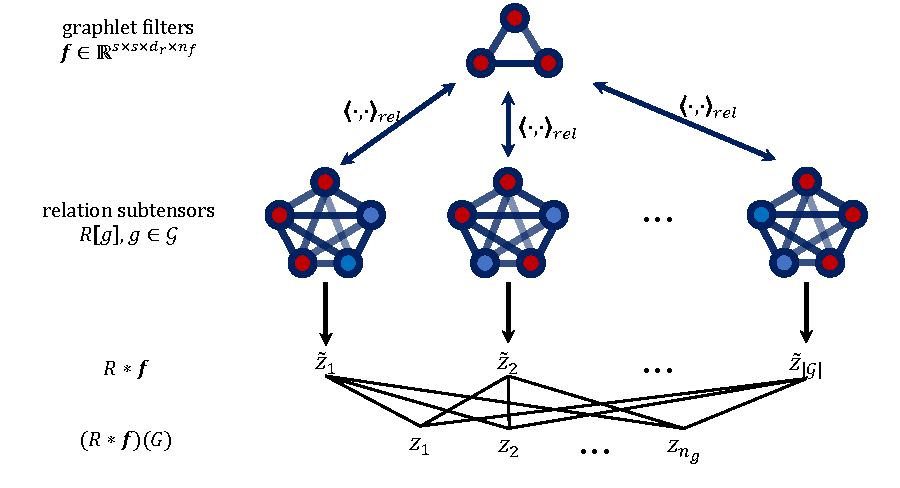
\includegraphics[width=0.9\textwidth]{figs/relconv_diagram2.pdf}
    \vskip-10pt
    \caption{A depiction of the relational convolution operation.
    % NOTE / TODO temporarily add? (reviewer asked for this but we're tight on space)
    % The input is a relation tensor $R \in \reals^{n \times n \times d_r}$. A learned set of graphlet filters $\bm{f} \in \reals^{s \times s \times d_r \times n_f}$ are compared to each relation subtensor $R[g], g \in \calG$, producing the relational convolution $R \ast \bm{f}$. With a group matrix $G \in \reals^{m \times n_g}$, $(R \ast \bm{f})(G)$ represents the relational information in a set of $n_g$ ``soft groups''.
    % The input is a relation tensor $R$ of shape $m \times m \times d_r$, giving pairwise relations of dimension $d_r$ between a sequence of $m$ objects. A graphlet filter of size $s$ is parameterized by a relation tensor of shape $s \times s \times d_r$. The graphlet convolution operation computes relational inner products between the relation subtensor of each discrete group $g \in \calG$ with the graphlet filters $\bm{f}$. This gives a vector representation of the relations in each discrete group, $\tilde{z}_g \in \reals^{n_f}, g \in \calG$. Finally, this is synthesized into a vector representation for each of $n_g$ `soft groups', $G$, producing $(R \ast \bm{f})(G) = (z_1, \ldots, z_{n_g})$.
    }\label{fig:relconvdiagram}
    \vskip -10pt
\end{figure}

\subsection{Relational convolutions with `soft' groups}

In the above formulation, the groups are `discrete'. Having discrete groups can be desirable for interpretability, if the relevant groupings are known a priori or if considering every possible grouping is computationally and statistically feasible. However, if the relevant groupings are not known, then considering all possible combinations results in a rapid growth of the number of objects at each layer.
% Besides being computationally intractable, considering every possible grouping may be unnecessary and may make learning more difficult.

In order to address these issues, we propose \textit{explicitly modeling groups}. This allows us to control the number of objects in the output sequence of a relational convolution operation such that only relevant groups are considered. In the next section, we outline some ways to model `soft groups' using \textit{grouping layers}. These layers take a sequence of objects and/or the relation tensor as input and produce a `group matrix' $G \in \reals^{n \times n_g}$ representing $n_g$ `soft groups'. The $(i,j)$-th entry of the group matrix represents the degree to which the $i$-th object belongs to the $j$-th group. The number of groups $n_g$ is a configurable hyperparameter of the grouping layers. For the remainder of this subsection, we assume that the group matrix $G$ is given as input to the relational convolution layer.

Consider the group matrix $G \in \reals^{n \times n_g}$ and filters $\bm{f}$ of size $s$. First, we use $G$ to compute a ``group-match score'' for each discrete group $g$ of size $s$ (e.g., $g \in \calG = \binom{[n]}{s}$). This is done via
\begin{equation}\label{eq:group_match_score}
    \begin{split}
        G &\gets \text{SoftPlus}(G)\\
        \alpha_{gk} &\gets \text{Normalize}\paren{\bra{\prod_{i \in g} G[i,k]}_{g \in \calG}}, \quad g \in \calG, k \in [n_g],
    \end{split}
\end{equation}
where the soft-plus function is $\text{Softplus}(x) = \log(\exp(x + 1))$, applied elementwise. This has the effect of making the group matrix $G$ non-negative which is needed for the product of its elements to represent a ``group-match score''. The product inside the softmax is over elements in the discrete group $g \in \calG$. Hence, it will be large whenever the soft group $G_k := G[:, k]$ aligns with the discrete group $g$. $\mathrm{Normalize}(\cdot)$ normalizes the group match scores so that $\sum_{g} \alpha_{gk} = 1$. We propose the use of sparse normalizers~\citep{lahaControllableSparseAlternatives2018a} so that only a sparse subset of discrete groups in $\calG$ contribute to each soft group (see also~\Cref{ssec:computational_considerations}). In our experiments, we use `sparsemax'~\citep{martinsSoftmaxSparsemaxSparse2016}. Thus, $\alpha_{gk}$ is a normalized ``group-match score'' indicating the degree to which the discrete group $g$ matches the given soft group $G_k$.
% \footnote{Sparse normalizers would likely be appropriate alternatives to softmax here, since it would be desirable to have only a sparse subset of discrete groups in $\calG$ contribute to each soft group. Some sparse alternatives to softmax are discussed in~\citep{lahaControllableSparseAlternatives2018a}.}. %Note that the group match scores of discrete groups sum to one, $\sum_{g \in G} \alpha_{gk} = 1, \ \forall k \in [n_g]$.

Now, we can define the `soft' relational inner product \textit{given} the soft group $G_k$ by
\begin{equation}\label{eq:soft_relational_inner_prod}
    \langle R, \boldsymbol{f} \, \vert \, G_k \rangle_R \coloneqq \sum_{g \in \calG} \alpha_{gk} \iprod{R[g]}{\boldsymbol{f}}_\mathrm{rel}.
\end{equation}
This notation should be read as ``the relational inner product of the relation tensor $R$ with the graphlet filters $\boldsymbol{f}$ given the group $G_k$''. This expression is essentially a convex combination of the relational inner product with all possible discrete groups weighted by how much they match the soft group $G_k$.

With this modification, the number of objects in the output sequence is fixed and controlled by the number of groups, $n_g$ (which is a hyperparameter). The output sequence of the relational convolution given groups $G$ is now given by
\begin{equation}\label{eq:soft_relational_convolution_groups}
    (R \ast \bm{f})(G) = \left( \softreliprod{R}{\bm{f}}{G_1}, \ldots, \softreliprod{R}{\bm{f}}{G_{n_g}} \right) \in \left(\mathbb{R}^{n_f}\right)^{n_g}.
\end{equation}

\subsection{Relational convolutions with group attention \textcolor{red}{[ALTERNATIVE]}}

In the above formulation, the groups are `discrete'. Having discrete groups can be desirable for interpretability, if the relevant groupings are known a priori or if considering every possible grouping is computationally and statistically feasible. However, if the relevant groupings are not known, then considering all possible combinations results in a rapid growth of the number of objects at each layer.
% Besides being computationally intractable, considering every possible grouping may be unnecessary and may make learning more difficult.

In order to address these issues, we propose \textit{explicitly modeling groups}. This allows us to control the number of objects in the output sequence of a relational convolution operation such that only relevant groups are considered. We propose modeling groups via an \textit{attention} operation.

Consider the input $X = \paren{x_1, \ldots, x_n},\, x_i \in \reals^d$. Let $n_g$ be the number of groups to be learned and $s$ be the size of the graphlet filter, which are hyperparameters to the model. We learn $n_g \times s$ group query vectors $Q = \{q_{i}^{g}\}_{g \in [n_g], i \in [s]}$. That is, for each group $g \in [n_g]$, we learn $s$ queries which will be used to retrieve a group of size $s$ via attention. The $i$-th object in the $k$-th group is retrieved via an attention operation as follows,
\begin{equation}\label{eq:group_attn}
    \begin{aligned}
        \bar{x}_{i}^{g} &= \sum_{j = 1}^{n} \alpha_{ij}^{g} x_j, \ &&g \in [n_g],  i \in [s]\\
        \alpha_{ij}^{g} &= \frac{\exp\paren{\beta \iprod{q_i^g}{\mathtt{key}(x_j)}}}{\sum_{k = 1}^{n}{\exp\paren{\beta \iprod{q_i^g}{\mathtt{key}(x_k)}}}}, \ &&k \in [n_g], i \in [s], j \in [n]
    \end{aligned}
\end{equation}
where $\bar{x}_{i}^{g}$ is the $i$-th object in the $g$-th group, $q_{i}^{g}$ is the query for retrieving the $i$-th object in the $g$-th group, $\mathtt{key}(x_j)$ is the key associated with the object $x_j$, and $\beta$ is a learnable scaling parameter.

The $\mathtt{key}$ for each object is computed as a function of its position, features, and/or context. For example, to group objects based on their position, the key can be a positional embedding. To group based on features, the $\mathtt{key}$ can be a linear projection of the object's feature vector. To group based on both position and features, the $\mathtt{key}$ can be a sum or concatenation of the above. Finally, groups can also be modeled based on contextual information by computing keys through a self-attention operation.

\Cref{eq:group_attn} can be computed in parallel with an `einsum' operation in $\calO(n \cdot n_g \cdot s \cdot d)$ operations. When the hyperparameters of the model are fixed, this is linear in the sequence length $n$.

The relation subtensor $\bar{R}[g] \in \reals^{s \times s \times d_r}$ for each group $g \in [n_g]$ is then computed using a shared MD-IPR layer $r(x, y)$,
\begin{equation}
    \bar{R}[g]_{ij} = r(\bar{x}_{i}^{g}, \bar{x}_{j}^{g}).
\end{equation}
This computation can be carried out in parallel via efficient matrix multiplication with $\calO(n_g \cdot s^2 \cdot d_r \cdot d_{\mathrm{proj}})$ operations. Note that This does not scale with the number of objects in the input, and is only a function of the hyperparameters of the model. Moreover, the filter size $s$ is typically of very modest size (e.g., $3$ or $5$).

The relational convolution is computed as before via,
\begin{equation}
    \bar{R} \ast \bm{f} \equiv \paren{\reliprod{\bar{R}[g]}{\bm{f}}}_{g \in [n_g]}.
\end{equation}

Overall, relational convolution with group attention can be summarized as follows: 1) learn $n_g$ groupings of objects, retrieving $s$ objects per group; 2) compute the relation tensor of each group using a MD-IPR module; 3) compute a relational convolution with a learned set of graphlet filters $\bm{f}$, producing a sequence of $n_g$ vectors each describing the relational pattern within a (learned) group of objects.

The group attention scores in~\Cref{eq:group_attn} are ideally close to discrete assignments. That is, the vector $\alpha_{i,\cdot}^{g} \in \Delta^{n}$ is ideally a one-hot vector for each $g \in [n_g],\, i \in [s]$. To encourage the model to learn more structured group assignments, we add an entropy regularization to the loss function, $\calL_{\mathtt{entr}} = \frac{1}{n_g \cdot s} \sum_{g, i} H(\alpha_{i,\cdot}^{g})$, where $H(\alpha_{i,\cdot}^{g}) = - \sum_{j} \alpha_{ij}^{g} \log(\alpha_{ij}^g)$ is the Shannon entropy. As a heuristic, this regularization can be scaled by $\sim \log(\mathtt{n\_classes}) / \log(n)$ so that it doesn't dominate the underlying task's loss.

% \section{Grouping Layers}\label{sec:grouping_layers}

A grouping layer is a layer which outputs a group matrix $G \in \reals^{m \times n_g}$ representing the degree to which each object $i \in [m]$ belongs to each group $j \in [n_g]$. The number of groups $n_g$ is a configurable hyperparameter. We briefly describe some proposals for grouping layers with different properties.

\textbf{Temporal Grouping.} In the temporal grouping layer, the groups are a function only of the temporal order of the objects. This can be achieved by learning the group matrix $G$ directly as a parameter of the model. $G$ will be optimized along with the rest of the model parameters as a function of its effect on the relational convolution layer. Temporal grouping would be appropriate in situations where the order in which objects appear is predetermined and indicates the relevant groups.

\textbf{Feature-based Grouping.} In a feature-based grouping layer, the group(s) to which each object belongs is a function of that object's features (and position). That is,
\begin{equation}
        G \gets \begin{bmatrix}
            \phi(1, x_1)^\top \\
            \vdots \\
            \phi(m, x_m)^\top
        \end{bmatrix} \in \reals^{m \times n_g},
\end{equation}

\noindent where $\phi: [m] \times \calX \to \reals^{n_g}$ is a learnable function which maps an object's temporal order $i$ and feature representation $x_i$ to a $n_g$-dimensional group membership vector where the $j$th entry of the vector represents the degree to which the object belongs to the $j$th group. For example $\phi$ can be a multi-layer perceptron of the form $\phi(i, x) = \mathrm{MLP}(\mathrm{concat}(e_i, x))$. Feature-based grouping may be useful in situations where group membership can be determined for each object using only that object's features, irrespective of the context of the other objects in the sequence.

\textbf{Context-aware Grouping.} In some applications, the group(s) to which each object belongs to may depend on the full context of the other objects in the sequence. One way to model this is to use a message-passing neural network to update the representations of each object, incorporating the context of the other objects in the sequence. Then, a multi-layer perceptron is applied to each encoded object to produce the group membership vector for that object.
\begin{equation}
    \begin{split}
        E_i &\gets \mathrm{MessagePassing}\paren{x_i, \set{x_1, \ldots, x_m}}, \ i \in [m] \\
        G &\gets \begin{bmatrix}\mathrm{MLP}(E_1)^\top \\ \vdots \\ \mathrm{MLP}(E_m)^\top \end{bmatrix} \in \reals^{m \times n_g}.
    \end{split}
\end{equation}

This is the most general form of grouping, as it encompasses the previous two forms as special cases. The updated representation of each object $E_i$ now contains any relevant information about the other objects which should be considered in computing its group membership vector. One simple and effective option for the message-passing operation is to use self-attention. In this case, since a multi-head relational layer precedes the relational convolution layer, the relation tensor can be re-used in the self-attention operation to compute attention scores.

\section{Experiments}\label{sec:experiments}

\texttt{[TODO]}

\texttt{Description of relational games}

\begin{table}
    \centering
    \begin{tabular}{llll}
\toprule
              &             &     Hexos Accuracy &   Stripes Accuracy \\
Task & Model &                    &                    \\
\midrule
same & RelConvNet &  $0.989 \pm 0.002$ &  $0.974 \pm 0.003$ \\
              & CoRelNet &  $0.988 \pm 0.006$ &  $0.724 \pm 0.112$ \\
              & PrediNet &  $0.990 \pm 0.004$ &  $0.983 \pm 0.007$ \\
              & Transformer &  $0.997 \pm 0.001$ &  $0.993 \pm 0.004$ \\\hline
occurs & RelConvNet &  $0.980 \pm 0.001$ &  $0.880 \pm 0.015$ \\
              & CoRelNet &  $0.992 \pm 0.004$ &  $0.518 \pm 0.012$ \\
              & PrediNet &  $0.907 \pm 0.020$ &  $0.775 \pm 0.046$ \\
              & Transformer &  $0.881 \pm 0.015$ &  $0.724 \pm 0.021$ \\\hline
xoccurs & RelConvNet &  $0.967 \pm 0.001$ &  $0.946 \pm 0.006$ \\
              & CoRelNet &  $0.980 \pm 0.007$ &  $0.606 \pm 0.035$ \\
              & PrediNet &  $0.872 \pm 0.036$ &  $0.810 \pm 0.028$ \\
              & Transformer &  $0.867 \pm 0.017$ &  $0.753 \pm 0.031$ \\\hline
between & RelConvNet &  $0.991 \pm 0.001$ &  $0.988 \pm 0.002$ \\
              & CoRelNet &  $0.995 \pm 0.001$ &  $0.582 \pm 0.063$ \\
              & PrediNet &  $0.978 \pm 0.006$ &  $0.950 \pm 0.019$ \\
              & Transformer &  $0.986 \pm 0.003$ &  $0.961 \pm 0.010$ \\\hline
match pattern & RelConvNet &  $0.961 \pm 0.015$ &  $0.870 \pm 0.041$ \\
              & CoRelNet &  $0.942 \pm 0.011$ &  $0.581 \pm 0.026$ \\
              & PrediNet &  $0.710 \pm 0.040$ &  $0.658 \pm 0.053$ \\
              & Transformer &  $0.627 \pm 0.005$ &  $0.591 \pm 0.006$ \\
\bottomrule
\end{tabular}

    \caption{Out-of-distribution Generalization results on relational games.}
\end{table}


\section{Discussion}\label{sec:discussion}
% \textbf{Summary.} 
\subsection*{Summary}
In this paper, we proposed a compositional architecture and framework for learning hierarchical relational representations via a novel relational convolution operation. The relational convolution operation we propose here is a `convolution' in the sense that it considers a patch of the relation tensor, given by a group of objects, and compares the relations within it to a template graphlet filter via an appropriately-defined inner product. This is analogous to convolutional neural networks, where an image filter is compared against different patches of the input image. Moreover, we propose an attention-based mechanism for modeling useful groupings of objects in order to maintain scalability. By alternating inner product relation layers and relational convolution layers, we obtain an architecture that naturally models hierarchical relations.

% Since the same graphlet filters are used for all groupings, the relational convolution operation implements a form of \textit{parameter-sharing} which yields improved sample-efficiency and generalization. Another important feature of the relational convolution operation is its \textit{interpretability}. The graphlet filters $\bm{f} = (f_1, \ldots, f_{n_f})$ are each a particular pattern of relations between $s$ objects. Each object in the output of a relational convolution $R \ast \bm{f}$ represents the degree to which the relations in the group $g$ match the patterns in each filter.

%\aanote{This part is new.}
\subsection*{Discussion on relational inductive biases}
In our experiments, we observed that general-purpose sequence models like the Transformer struggle to learn tasks that involve relational reasoning in a data-efficient way. The relational inductive biases of RelConvNet, CoRelNet, and PrediNet result in significantly improved performance on the relational games tasks. These models each implement different kinds of relational inductive biases, and are each designed with different motivations in mind. For example, PrediNet's architecture is loosely inspired by the structure of predicate logic, but can be understood as ultimately producing representations of pairwise difference relations, with pairs of objects selected by an attention operation. CoRelNet is a minimal relational architecture that consists of computing an $n \times n$ inner product similarity matrix followed by a softmax normalization. RelConvNet, our proposed architecture, provides further flexibility across several dimensions. Like CoRelNet, it models relations as inner products of feature maps, but it achieves greater representational capacity by learning multi-dimensional relations through multiple learned feature maps or filters. More importantly, the relational convolutions operation enables learning higher-order relations between groups of objects. This is in contrast to both PrediNet and CoRelNet, which are limited to pairwise relations. Our experiments show that the inductive biases of RelConvNet result in improved performance in relational reasoning tasks. In particular, the \textit{SET} task, where RelConvNet was the only model able to generalize non-trivially, demonstrates the necessity for explicit inductive biases that support learning hierarchical relations.

% \textbf{Limitations and future work.} 
\subsection*{Limitations and future work}
The tasks considered here are solvable by modeling only second-order relations at most. We observe that the relational convolutional networks architecture saturates the relational games benchmark of~\citet{shanahanExplicitlyRelationalNeural}. While the ``contains set'' task demonstrates a sharp separation between relational convolutional networks and existing baselines, this task too only involves second-order relations.
% , and does not fully test the abilities of the framework. 
A more thorough evaluation of this architecture, and future architectures for modeling hierarchical relations, would require the development of new benchmark tasks and datasets that involve a larger number of objects and higher-order relations. This is a subtle and non-trivial task that we leave for future work.

The experiments considered here are synthetic relational tasks designed for a controlled evaluation. In more realistic settings, we envision relational convolutional networks as modules embedded in a broader architecture. For example, a relational convolutional network can be embedded into an RL agent to enable performing tasks involving relational reasoning. Similarly, relational convolutions can perhaps be integrated into general-purpose sequence models, such as Transformers, to enable improved relational reasoning while retaining the generality of the architecture.

\subsection*{Code and data}
Code and experimental logs are available at: \texttt{https://[Anonymized]}

% \medskip

% \clearpage
{%\small
\bibliography{references}
\bibliographystyle{iclr2024_conference}
}

\clearpage
\appendix

\section{Experiments Supplement}\label{sec:experiments_supplement}

\subsection{Relational Games (\Cref{ssec:exp_relational_games})}

The pentominoes split is used for training,
and the hexominoes and stripes splits are used to test out-of-distribution generalization after training. We hold out 1000 samples for validation (during training) and 5000 samples for testing (after training), and use the rest as the training set. We train for 50 epochs using the categorical cross-entropy loss and the Adam optimizer with learning rate $0.001$, $\beta_1 = 0.9, \beta_2 = 0.999, \epsilon = 10^{-7}$. We use a batch size of 512. For each model and task, we run 5 trials with different random seeds.\Cref{tab:relational_games_tasks} contains text descriptions of each task in the relational games dataset in the experiments of~\Cref{ssec:exp_relational_games}.~\Cref{tab:relgames_architectures} contains a description of the architectures of each model (or shared component) in the experiments.
% ~\Cref{tab:relgames_group_architectures} contains a description of the hyperparameters of the grouping layers corresponding to the `Temporal G', `Feature G', and `Contextual G' RelConvNet models. All grouping layers have 16 soft groups, and the normalizer in~\Cref{eq:group_match_score} is sparsemax.
\Cref{tab:ood_generalization} reports the accuracy on the hold-out object sets (i.e., the numbers depicted in~\Cref{fig:ood_generalization} of the main text).

\subsection{SET (\Cref{ssec:experiments_set})}

We train for 100 epochs using the categorical cross-entropy loss and the Adam optimizer with learning rate $0.001$, $\beta_1 = 0.9, \beta_2 = 0.999, \epsilon = 10^{-7}$. We use a batch size of 512. For each model and task, we run 5 trials with different random seeds.\Cref{tab:set_architectures} contains a description of the architecture of each model in the ``contains set'' experiments of~\Cref{ssec:experiments_set}.~\Cref{tab:set_acc} reports the generalization accuracies on the hold-out `sets' (i.e., the numbers depicted in~\Cref{fig:contains_set_acc} of the main text).

\begin{table}[H]
    \centering
    \begin{tabular}{p{0.2\textwidth}p{0.7\textwidth}}
    \toprule
    Task              & Description                                                                                                                                                                                             \\ \midrule
    \texttt{same}              & Two random cells out of nine are occupied by an object. They are the ``same'' if they have the same color, shape, and orientation (i.e., identical image)                                               \\\hline
    \texttt{occurs}            & The top row contains one object and the bottom row contains three objects. The ``occurs'' relationship holds if at least one of the objects in the bottom row is the same as the object in the top row. \\\hline
    \texttt{xoccurs}           & Same as occurs, but the relationship holds if exactly one of the objects in the bottom row is the same as the object in the top row.                                                                    \\\hline
    \texttt{between}           & The grid is occupied by three objects in a line (horizontal or vertical). The ``between'' relationship holds if the outer objects are the same.                                                         \\\hline
    \texttt{row match pattern} & The first and third rows of the grid are occupied by three objects each. The ``match pattern'' relationship holds if the relation pattern in each row is the same (e.g., AAA, AAB, ABC, etc.)           \\ \bottomrule
\end{tabular}
    \caption{Relational games tasks.}\label{tab:relational_games_tasks}
\end{table}

\begin{table}[H]
    \centering
    \begin{tabular}{p{0.25\textwidth}p{0.75\textwidth}}
    \toprule
    Model / Component & Architecture \\ \midrule
    Common CNN \newline Embedder & \texttt{Conv2D} $\to$ \texttt{MaxPool2D} $\to$ \texttt{Conv2D} $\to$ \texttt{MaxPool2D} $\to$ \texttt{Flatten}. \newline
                        \texttt{Conv2D}: num filters = 16, filter size = $3 \times 3$, activation = relu. \newline
                        \texttt{MaxPool2D}: stride = 2. \\\hline
    RelConvNet        & \texttt{CNN} $\to$ \texttt{MD-IPR} $\to$ \texttt{RelConv} $\to$ \texttt{Flatten} $\to$ \texttt{MLP}. \newline
                        \texttt{MD-IPR}: relation dim = 16, projection dim = 4, symmetric. \newline
                        \texttt{RelConv}: num filters = 16, filter size = 3, discrete groups = combinations. \\\hline
    CoRelNet          & \texttt{CNN} $\to$ \texttt{CoRelNet} $\to$ \texttt{Flatten} $\to$ \texttt{MLP}. \newline
                        Standard CoRelNet has no hyperparameters. \\\hline
    PrediNet          & \texttt{CNN} $\to$ \texttt{PrediNet} $\to$ \texttt{Flatten} $\to$ \texttt{MLP}. \newline
                        \texttt{PrediNet}: key dim = 4, number of heads = 4, num relations = 16. \\\hline
    Transformer       & \texttt{CNN} $\to$ \texttt{TransformerEncoder} $\to$ \texttt{AveragePooling} $\to$ \texttt{MLP}. \newline
                    \texttt{TransformerEncoder}: num layers = 1, num heads = 8, feedforward intermediate size = 32, activation = relu. \\\hline
    GCN               &
        \texttt{CNN} $\to$ \texttt{AddPosEmb} $\to$ (\texttt{GCNConv} $\to$ \texttt{Dense}) $\times 2$ $\to$ \texttt{AveragePooling} $\to$ \texttt{MLP}. \newline
        \texttt{GCConv}: channels = 128, \texttt{Dense}: num neurons = 128, activation = relu \\\hline
    GAT               &
        \texttt{CNN} $\to$ \texttt{AddPosEmb} $\to$ (\texttt{GATConv} $\to$ \texttt{Dense}) $\times 2$ $\to$ \texttt{AveragePooling} $\to$ \texttt{MLP}. \newline
        \texttt{GATonv}: channels = 128, \texttt{Dense}: num neurons = 128, activation = relu \\\hline
    GCN               &
        \texttt{CNN} $\to$ \texttt{AddPosEmb} $\to$ (\texttt{GINConv} $\to$ \texttt{Dense}) $\times 2$ $\to$ \texttt{AveragePooling} $\to$ \texttt{MLP}. \newline
        \texttt{GINConv}: channels = 128, \texttt{Dense}: num neurons = 128, activation = relu \\\hline
                Common output MLP & \texttt{Dense(64, `relu')} $\to$ \texttt{Dense(2)}. \\ \bottomrule
\end{tabular}
    \caption{Model architectures for relational games experiments.}\label{tab:relgames_architectures}
\end{table}

\begin{table}[H]
    \centering
    \begin{tabular}{llll}
\toprule
              &             &     Hexos Accuracy &   Stripes Accuracy \\
Task & Model &                    &                    \\
\midrule
same & RelConvNet &  $0.989 \pm 0.002$ &  $0.974 \pm 0.003$ \\
              & CoRelNet &  $0.988 \pm 0.006$ &  $0.724 \pm 0.112$ \\
              & PrediNet &  $0.990 \pm 0.004$ &  $0.983 \pm 0.007$ \\
              & Transformer &  $0.997 \pm 0.001$ &  $0.993 \pm 0.004$ \\\hline
occurs & RelConvNet &  $0.980 \pm 0.001$ &  $0.880 \pm 0.015$ \\
              & CoRelNet &  $0.992 \pm 0.004$ &  $0.518 \pm 0.012$ \\
              & PrediNet &  $0.907 \pm 0.020$ &  $0.775 \pm 0.046$ \\
              & Transformer &  $0.881 \pm 0.015$ &  $0.724 \pm 0.021$ \\\hline
xoccurs & RelConvNet &  $0.967 \pm 0.001$ &  $0.946 \pm 0.006$ \\
              & CoRelNet &  $0.980 \pm 0.007$ &  $0.606 \pm 0.035$ \\
              & PrediNet &  $0.872 \pm 0.036$ &  $0.810 \pm 0.028$ \\
              & Transformer &  $0.867 \pm 0.017$ &  $0.753 \pm 0.031$ \\\hline
between & RelConvNet &  $0.991 \pm 0.001$ &  $0.988 \pm 0.002$ \\
              & CoRelNet &  $0.995 \pm 0.001$ &  $0.582 \pm 0.063$ \\
              & PrediNet &  $0.978 \pm 0.006$ &  $0.950 \pm 0.019$ \\
              & Transformer &  $0.986 \pm 0.003$ &  $0.961 \pm 0.010$ \\\hline
match pattern & RelConvNet &  $0.961 \pm 0.015$ &  $0.870 \pm 0.041$ \\
              & CoRelNet &  $0.942 \pm 0.011$ &  $0.581 \pm 0.026$ \\
              & PrediNet &  $0.710 \pm 0.040$ &  $0.658 \pm 0.053$ \\
              & Transformer &  $0.627 \pm 0.005$ &  $0.591 \pm 0.006$ \\
\bottomrule
\end{tabular}

    \caption{Out-of-distribution generalization results on relational games. We report means $\pm$ standard error of mean over 5 trials. These are the numbers associated with~\Cref{fig:ood_generalization}.}\label{tab:ood_generalization}
\end{table}

\begin{table}[H]
    \centering
    \begin{tabular}{p{0.25\textwidth}p{0.75\textwidth}}
    \toprule
    Model / Component & Architecture                                                                                                                                                                                                                                                                                       \\ \midrule
    Common CNN \newline Embedder & 
        \texttt{Conv2D} $\to$ \texttt{MaxPool2D} $\to$ \texttt{Conv2D} $\to$ \texttt{MaxPool2D} $\to$ \texttt{Flatten} $\to$ \texttt{Dense(64, 'relu') $\to$ \texttt{Dense(64, 'tanh')}}. \newline
        \texttt{Conv2D}: num filters = 32, filter size = $5 \times 5$, activation = relu. \newline
        \texttt{MaxPool2D}: stride = 4. \\\hline
    RelConvNet        & 
        \texttt{CNN} $\to$ \texttt{MD-IPR} $\to$ \texttt{RelConv} $\to$ \texttt{Flatten} $\to$ \texttt{MLP}. \newline
        \texttt{MD-IPR}: relation dim = 16, projection dim = 16, symmetric. \newline
        \texttt{RelConv}: num filters = 16, filter size = 3, discrete groups = combinations, symmetric relational inner product with `max' aggregator. \\\hline
    CoRelNet          &
        \texttt{CNN} $\to$ \texttt{CoRelNet} $\to$ \texttt{Flatten} $\to$ \texttt{MLP}. \newline
        Standard CoRelNet has no hyperparameters. \\\hline
    PrediNet          &
        \texttt{CNN} $\to$ \texttt{PrediNet} $\to$ \texttt{Flatten} $\to$ \texttt{MLP}. \newline
        \texttt{PrediNet}: key dim = 4, number of heads = 4, num relations = 16. \\\hline
    Transformer       & 
        \texttt{CNN} $\to$ \texttt{TransformerEncoder} $\to$ \texttt{AveragePooling} $\to$ \texttt{MLP}. \newline
        \texttt{TransformerEncoder}: num layers = 1, num heads = 8, feedforward intermediate size = 32, activation = relu. \\\hline
    GCN               &
        \texttt{CNN} $\to$ (\texttt{GCNConv} $\to$ \texttt{Dense}) $\times 2$ $\to$ \texttt{AveragePooling} $\to$ \texttt{MLP}. \newline
        \texttt{GCConv}: channels = 128, \texttt{Dense}: num neurons = 128, activation = relu \\\hline
    GAT               &
        \texttt{CNN} $\to$ (\texttt{GATConv} $\to$ \texttt{Dense}) $\times 2$ $\to$ \texttt{AveragePooling} $\to$ \texttt{MLP}. \newline
        \texttt{GATonv}: channels = 128, \texttt{Dense}: num neurons = 128, activation = relu \\\hline
    GCN               &
        \texttt{CNN} $\to$ (\texttt{GINConv} $\to$ \texttt{Dense}) $\times 2$ $\to$ \texttt{AveragePooling} $\to$ \texttt{MLP}. \newline
        \texttt{GINConv}: channels = 128, \texttt{Dense}: num neurons = 128, activation = relu \\\hline
    Common output MLP & \texttt{Dense(64, `relu')} $\to$ \texttt{Dense(32, `relu')} $\to$ \texttt{Dense(2)}. \\ \bottomrule
\end{tabular}
    \caption{Model architectures for ``contains set'' experiments.}\label{tab:set_architectures}
\end{table}

\begin{table}[H]
    \centering
    \begin{tabular}{ll}
\toprule
{} &           Accuracy \\
Model       &                    \\
\midrule
RelConvNet  &  $0.979 \pm 0.006$ \\
CoRelNet    &  $0.563 \pm 0.001$ \\
PrediNet    &  $0.508 \pm 0.002$ \\
Transformer &  $0.584 \pm 0.004$ \\
GCN         &  $0.595 \pm 0.003$ \\
GAT         &  $0.517 \pm 0.015$ \\
GIN         &  $0.590 \pm 0.003$ \\
LSTM        &  $0.602 \pm 0.003$ \\
GRU         &  $0.593 \pm 0.004$ \\
\bottomrule
\end{tabular}

    \caption{Hold-out test accuracy on ``contains set'' task. We report means $\pm$ standard error of mean over 10 trials. These are the numbers associated with~\Cref{fig:contains_set_acc}.}\label{tab:set_acc}
\end{table}
\null
\vfill
\section{Computational efficiency and parameter efficiency}\label{sec:appendix_comp_param_efficiency}
\subsection{Parameter efficiency}\label{ssec:appendix_param_efficiency}

The parameter count of both MD-IPR and relational convolution layers does not scale with the number of input objects or the number of groups considered. Instead, the parameters are shared across objects and groups. This has computational and statistical benefits. In particular, it reduces memory usage and the number of weight updates during backpropagation, as well as making the statistical estimation of a good choice of parameters easier.

\textbf{MD-IPR layer.} In a multi-dimensional inner product relation module, the parameters are the left and right projection maps, $W_1^{(k)}, W_2^{(k)} \in \reals^{d_{\mathrm{proj}} \times d_{\mathrm{in}}}, k = 1, \ldots, d_r$, where the projection dimension $d_{\mathrm{proj}}$ and the relation dimension $d_r$ are hyperparameters, and $d_{\mathrm{in}}$ is the dimensionality of the input objects (~\Cref{eq:relation_function_lin_proj}). Hence, the parameter count of a MD-IPR layer is $d_r \times d_{\mathrm{proj}} \times d_{\mathrm{in}}$. Observe that while this scales with the dimensionality of the input objects $d_{\mathrm{in}}$, it does not scale with the number of objects $m$---the same encoders are shared across all pairs of objects.

\textbf{Relational Convolution layer.} The parameters in a relational convolution layer are the graphlet filters $\bm{f} \in \reals^{s \times s \times d_r \times n_f}$. Observe that the parameter count is independent of the number of groups $\abs{\calG}$ or even the number of objects $m$. The same graphlet filters are applied to the relation subtensor corresponding to each grouping of objects. This is similar to how convolutional neural networks apply the same filters to all patches of an image. The parameter count of a relational convolution layer depends only on the filter size and number of filters, which are hyperparameters.

\subsection{Computational considerations}\label{ssec:computational_considerations}

The MD-IPR module computes an $m \times m$ relation tensor, where $m$ is the number of input objects. This quadratic computational and memory cost can be avoided under assumptions of sparsity in the discrete groups $\calG$ or group assignment matrix $G$. Such optimizations will be useful in problems involving a large number of objects.

Consider first the case relational convolution with discrete groups. The output of the relational convolution layer is $R \ast \bm{f} = \paren{\reliprod{R[g]}{\bm{f}}}_{g \in \calG}$. For each $g \in \calG$, $R[g]$ encodes the relations between objects inside of $g$. Hence, rather than computing the full $m \times m$ relation tensor, we can instead compute only,
\begin{equation*}
    \calR := \set{R_{ij} \colon \exists\, g \in \calG \text{ such that } i,j \in g}.
\end{equation*}
When $\calG$ is sparse and structured, $\calR$ is sparse.

In the case of learned (soft) groups, the same computational benefits can be via a sparse selection in the group match score $\alpha_{gk}$ (~\Cref{eq:group_match_score}). This is achieved with sparse normalizers like sparsemax or top-$k$ softmax, for example. Then, the relation between object $i$ and object $j$ only needs to be computed if there exists a soft group $G_k, k \in [n_g]$ which assigns non-zero weight to a discrete $g \in \calG$ which includes both $i$ and $j$. That is,
\begin{equation*}
    \calR := \set{R_{ij} \colon \exists\, k \in [n_g], g \in \calG \text{ such that } \alpha_{gk} > 0 \text{ and } i,j \in g}.
\end{equation*}
Thus, only a sparse subset of the $m \times m$ relation tensor would need to be computed and stored.
\section{Geometry of representations learned by MD-IPR and Relational Convolutions}\label{sec:appendix_rep_analysis}

In this section, we explore and visualize the representations learned by MD-IPR and RelConv layers. In particular, we will visualize the representations produced by the RelConvNet model trained on the \textit{Set} task described in~\Cref{ssec:experiments_set}. Recall that the MD-IPR layer learns encoders $\phi_1, \psi_1, \ldots, \phi_{d_r}, \psi_{d_r}$. In this model $d_r = 16$, $\phi_i = \psi_i$ (so that learned relations are symmetric), and each $\phi_i$ is a linear transformation to $d_{\mathrm{proj}} = 4$-dimensional space. The representations learned by a selection of 6 encoders is visualized in~\Cref{fig:mdirp_encoders_rep}. For each of the 81 possible \textit{Set} cards, we apply each encoder in the MD-IPR layer, reduce to 2-dimensions via PCA, and visualize how each encoder separates the 4 attributes: number, color, fill, and shape. Observe, for example, that ``Encoder 0'' disentangles color and shape, ``Encoder 2'' disentangles fill, and ``Encoder 3'' disentangles number.

Next, we visualize, we explore the geometry of learned representations of relation vectors. That is, the inner products producing the 16-dimensional relation vector for each pair of objects. For each $\binom{81}{2}$ pairs of \textit{Set} cards, we compute the 16-dimensional relation vector learned by the MD-IPR layer, reduce to 2 dimensions via PCA, and visualize how the learned relation disentangles the latent same/different relations among the four attributes. This is shown in~\Cref{fig:mdipr_rel_rep}. We see some separation of the underlying same/different relations among the four attributes, even with only two dimensions out of 16.

Finally, we visualize the representations learned by the relational convolution layer. Recall that this layer learns a set of graphlet filters $\bm{f} \in \reals^{s \times s \times d_r \times n_f}$ which form templates of relational patterns against which groups of objects are compared. In our experiments, the filter size is $s = 3$ and the number of filters is $n_f = 16$. Hence, for each group $g$ of 3 \textit{Set} cards, the relational convolution layer produces a 16-dimensional vector, $\reliprod{R[g]}{\bm{f}} \in \reals^{n_f}$, summarizing the relational structure of the group. Of the $\binom{81}{3}$ possible triplets of \textit{Set} cards, we create a balanced sample of ``sets'' and ``non-sets''. We then compute $\reliprod{R[g]}{\bm{f}}$ and reduce to 2 dimensions via PCA.~\Cref{fig:conv_rep} strikingly shows that the representations learned by the relational convolution layer very clearly separate triplets of cards which form a set from those that don't form a set.


\begin{figure}
    \centering
    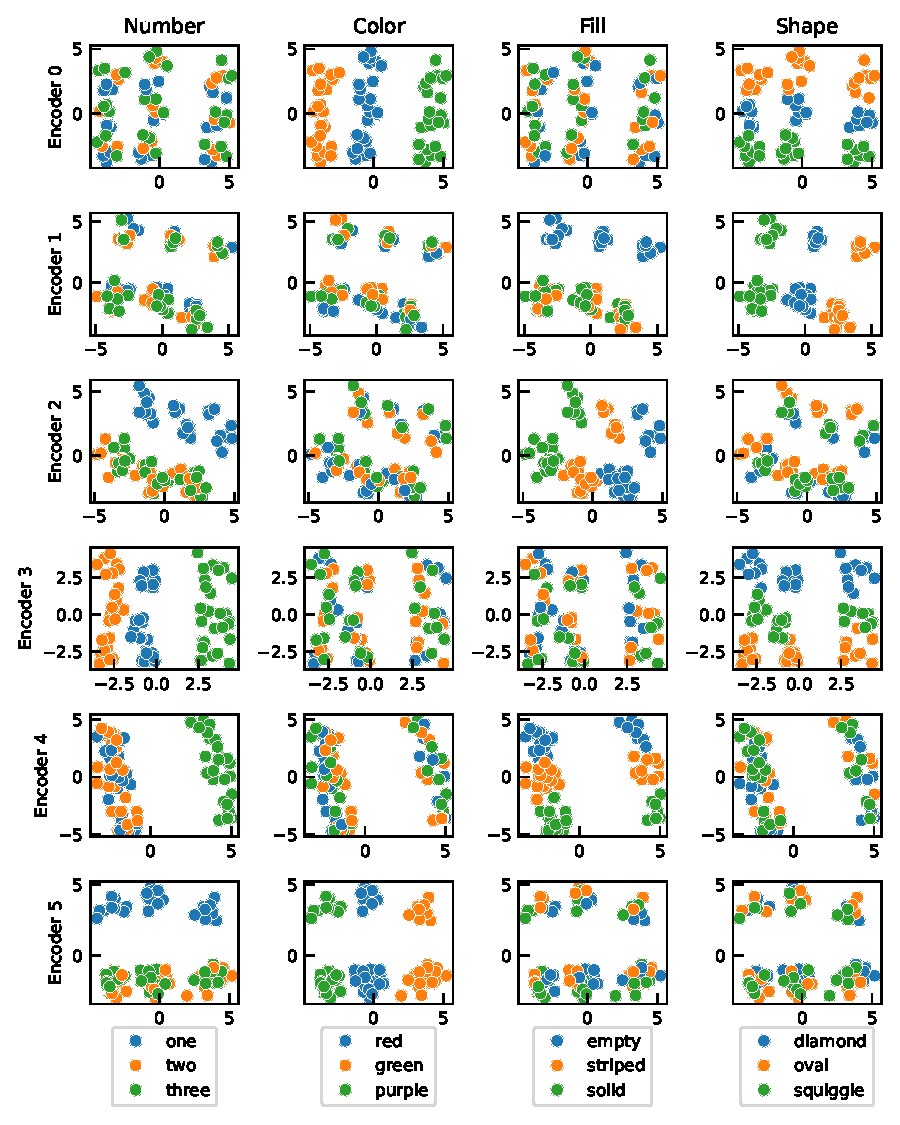
\includegraphics[width=0.9\textwidth]{figs/representation_analysis/mdipr_encoders_rep.pdf}
    \caption{The encoders learned in the MD-IPR layer represent the latent attributes in the \textit{Set} cards, with different encoders seemingly specializing to encode one or two attributes.}\label{fig:mdirp_encoders_rep}
\end{figure}

\begin{figure}
    \centering
    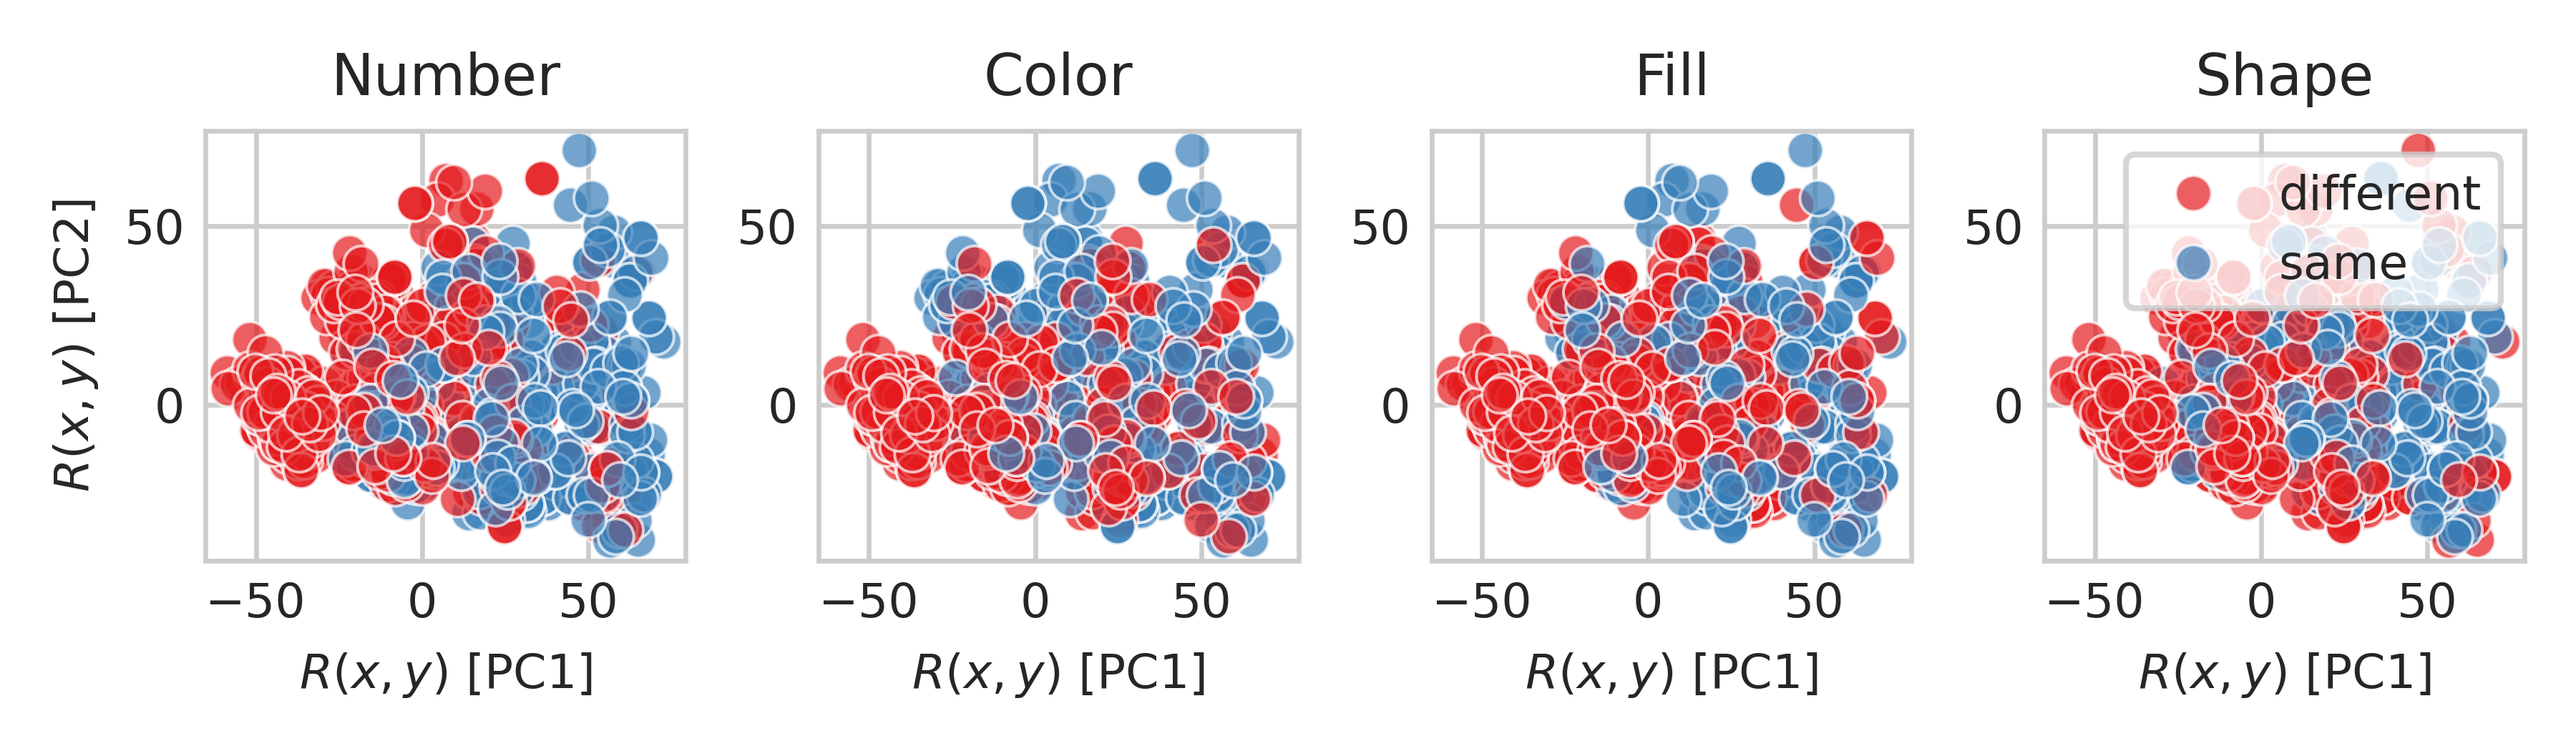
\includegraphics[width=0.95\textwidth]{figs/representation_analysis/mdipr_rel_rep.png}
    \caption{The relations learned by the MD-IPR layer encodes the latent relations underlying the \textit{Set} task.}\label{fig:mdipr_rel_rep}
\end{figure}

\begin{figure}
    \centering
    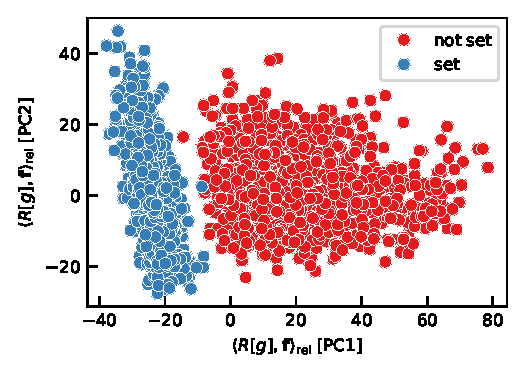
\includegraphics{figs/representation_analysis/conv_rep.pdf}
    \caption{The relational convolution layer produces representations which separates `sets' from `non-sets'.}\label{fig:conv_rep_appdx}
\end{figure}

% \null
% \vfill

\section{Some initial ideas on higher-order relational tasks}

As noted in the discussion, the tasks considered in this paper are solvable by modeling second-order relations at most. One of the main innovations of the relational convolutions architecture over existing relational architectures is its compositionality and ability to model higher-order relations. An important direction of future research is to test the architecture's ability to model hierarchical relations of increasing order. Constructing such benchmarks is a non-trivial task which requires careful thought and consideration. This was outside the scope of this paper, but we provide an initial discussion here which may be useful for constructing such benchmarks in future work.

\textbf{Propositional logic.} Consider a evaluating boolean logic formula such as, 
\begin{equation*}
    x_1 \land \paren{(x_2 \lor x_3) \land \paren{(\lnot x_3 \land x_4) \lor (x_5 \land x_6 \land x_7)}}.
\end{equation*}
Evaluating this logical expression (in this form) requires iteratively grouping objects and computing the relations between. For instance, we begin by computing the relation within $g_1 = (x_3, x_4)$ and the relation within $g_2 = (x_5, x_6, x_7)$, then we compute the relation between the groups $g_1$ and $g_2$, etc. For a task which involves logical reasoning of this hierarchical form, one might imagine the grouping layers in RelConvNet learning the relevant groups and the relational convolution operation computing the relations within each group. Taking inspiration from logical reasoning with such hierarchical structure may lead to interesting benchmarks of higher-order relational representation.

\textbf{Sequence modeling.} In sequence modeling (e.g., language modeling), modeling the relations between objects is usually essential. For example, syntactic and semantic relations between words are crucial to parsing language. Higher-order relations are also important, capturing syntactic and semantic relational features across different locations in the text and across multiple length-scales and layers of hierarchy~\citep[see for example some relevant work in linguistics][]{frank2012hierarchical,rosario2002descent}. The attention matrix in Transformers can be thought of as implicitly representing relations between tokens. It is possible that composing Transformer layers also learns hierarchical relations. However, as shown in this work and previous work on relational representation, Transformers have limited efficiency in representing relations. Thus, incorporating relational convolutions into Transformer-based sequence models may yield meaningful improvements in the relational aspects of sequence modeling. One way to do this is by cross-attending to a the sequence of relational objects produced by relational convolutions, each of which summarizes the relations within a group of objects at some level of hierarchy.

\textbf{Set embedding.} The objective of set embedding is to map a collection of objects to a euclidean vector which represents the important features of the objects in the set~\citep{zaheer2017deep}. Depending on what the set embedding will be used for, it may need to represent a combination of object-level features and relational information, including perhaps relations of higher order. A set embedder which incorporates relational convolutions may be able to generate representations which summarize relations between objects at multiple layers of hierarchy.

\textbf{Visual scene understanding.} In a visual scene, there are typically several objects with spatial, visual, and semantic relations between them which are crucial for parsing the scene. The CLEVR benchmark on visual scene understanding~\citep{johnson2017clevr} was used in early work on relational representation~\citep{santoroSimpleNeural2017}. In more complex situations, the objects in the scene may fall into natural groupings, and the spatial, visual, and semantic relations between those \textit{groups} may be important for parsing a scene (e.g., objects forming components with functional dependence). Integrating relational convolutions into a visual scene understanding system may enable reasoning about such higher-order relations.
\section{Discussion on use of TCN in evaluating relational architectures}\label{sec:appendix_tcn_discussion}

In~\Cref{ssec:exp_relational_games} the CoRelNet model of~\citet{kergNeuralArchitecture2022} was among the baselines we compared to. In that work, the authors also evaluate their model on the relational games benchmark. A difference between their experimental set up and ours is that they use a method called ``context normalization'' as a preprocessing step on the sequence of objects.

``Context normalization'' was proposed by~\citet{webbLearningRepresentationsThat2020}. The proposal is simple: Given a sequence of objects, $(x_1, \ldots, x_m)$, and a set of context windows $\calW_1, \ldots, \calW_W \subset \set{1, \ldots, m}$ which partition the objects, each object is normalized along each dimension with respect to the other objects in its context. That is, $\paren{z_1, \ldots, z_m} = \mathrm{CN}(x_1, \ldots, x_m)$ is computed as,
\begin{eqnarray*}
    \begin{split}
        \mu_j^{(k)} &= \frac{1}{\abs{\calW_k}} \sum_{t \in \calW_k} (x_t)_j\\
        \sigma_j^{(k)} &= \sqrt{ \frac{1}{\abs{\calW_k}} \sum_{t \in \calW_k} \paren{(x_t)_j - \mu_j^{(k)}}^2 + \varepsilon}\\
        (z_t)_j &= \gamma_j \paren{\frac{(x_t)_j - \mu_j^{(k)}}{\sigma_j^{(k)}}} + \beta_j, \qquad \text{for } t \in \calW_k
    \end{split}
\end{eqnarray*}
where $\gamma = (\gamma_1, \ldots, \gamma_d), \beta = (\beta_1, \ldots, \beta_d)$ are learnable gain and shift parameters for each dimension (initialized at 1 and 0, respectively, as with batch normalization). The context windows represent logical groupings of objects that are assumed to be known. For instance,~\citep{webbEmergentSymbols2021,kergNeuralArchitecture2022} consider a ``relational match-to-sample'' task where 3 pairs of objects are presented in sequence, and the task is to identify whether the relation in the first pair is the same as the relation in the second pair or the third pair. Here, the context windows would be the pairs of objects. In the relational games ``match rows pattern'' task, the context windows would be each row.

It is reported in~\citep{webbEmergentSymbols2021,kergNeuralArchitecture2022} that context normalization significantly accelerates learning and improves out-of-distribution generalization. Since~\citep{webbEmergentSymbols2021,kergNeuralArchitecture2022} use context normalization in their experiments, in this section we aim to explain our choice to exclude it. We argue that context normalization is a confounder and that an evaluation of relational architectures without such preprocessing is more informative.

To understand how context normalization works, consider first a context window of size 2, and let $\beta = 0, \gamma = 1$. Then, along each dimension, we have
\begin{align*}
    % \begin{split}
        \mathrm{CN}(x, x) &= \paren{0, 0},\\
        \mathrm{CN}(x, y) &= \paren{\mathrm{sign}(x - y), \mathrm{sign}(y - x)}.
    % \end{split}
\end{align*}
In particular, what context normalization does when there are two objects is, along each dimension, output 0 if the values is the same, and $\pm 1$ if it is different (encoding whether it is larger or smaller). Hence, it makes the context-normalized output independent of the original feature representation. For tasks like relational games, where the key relation to model is same/different, this preprocessing is directly encoding this information in a ``symbolic'' way. In particular, for two objects $x_1, x_2$, context normalized to produce $z_1, z_2$, we have that $x_1 = x_2$ if and only if $\iprod{z_1}{z_2} = 0$. This makes out-of-distribution generalization trivial, and does not properly test a relational architecture's ability to model the same/different relation.

Similarly, consider a context window of size 3. Then, along each dimension, we have,
\begin{align*}
    % \begin{split}
        \mathrm{CN}(x, x, x) &= \paren{0, 0, 0},\\
        \mathrm{CN}(x, x, y) &= \paren{\frac{1}{\sqrt{2}} \mathrm{sign}(x - y), \frac{1}{\sqrt{2}} \mathrm{sign}(x - y), \frac{1}{\sqrt{2}} \mathrm{sign}(y - x)}.
    % \end{split}
\end{align*}
Again, context normalization symbolically encodes the relational pattern. For any triplet of objects, regardless of the values they take, context normalization produces identical output in the cases above. With context windows larger than 3, the behavior becomes more complex.

These properties of context normalization make it a confounder in the evaluation of relational architectures. In particular, for small context windows especially, context normalization symbolically encodes the relevant information. Experiments on relational architectures should evaluate the architectures' ability to \textit{learn} those relations from data. Hence, we do not use context normalization in our experiments.


\end{document}